\section{Detection Findings}
\label{sec:results}

\begin{table*}[t]
\centering
\small
\begin{tabular}{llcccc}
\toprule
Method & Family & Overall & Within-bin & Matched-pair & Residual \\
\midrule
\multicolumn{2}{l}{\emph{Position-only}} & 0.830 & --- & --- & --- \\
\midrule
NLL            & Uncertainty    & 0.711 & 0.636 & 0.652 & 0.630 \\
Entropy        & Uncertainty    & 0.721 & 0.637 & 0.654 & \textbf{0.634} \\
IC             & Representation & 0.776 & \textbf{0.686} & \textbf{0.703} & 0.633 \\
GLSim          & Representation & 0.723 & 0.541 & 0.556 & 0.565 \\
GLSim (global) & Representation & 0.620 & 0.506 & 0.505 & 0.511 \\
GLSim (local)  & Representation & 0.772 & 0.564 & 0.593 & 0.601 \\
SVAR           & Attention      & 0.834 & 0.575 & 0.576 & 0.557 \\
PAS            & Attention      & \textbf{0.835} & 0.593 & 0.583 & 0.569 \\
Beyond-ADS     & Patch grounding& 0.503 & 0.511 & 0.515 & 0.501 \\
Beyond-CGC     & Patch grounding& 0.692 & 0.521 & 0.520 & 0.518 \\
Beyond-ADS+CGC & Patch grounding& 0.693 & 0.523 & 0.524 & 0.521 \\
\bottomrule
\end{tabular}
\caption{Overall vs.\ position-controlled AUROC on LLaVA-1.5-7B / MSCOCO ($16{,}426$ mentions). Generation position alone reaches $0.830$. Attention-mass detectors (PAS, SVAR) have the highest overall AUROC but collapse under position control; representation/uncertainty detectors (IC, Entropy, NLL) remain robust. Best per column in \textbf{bold}.}
\label{tab:main}
\end{table*}



\begin{figure*}[t]
\centering
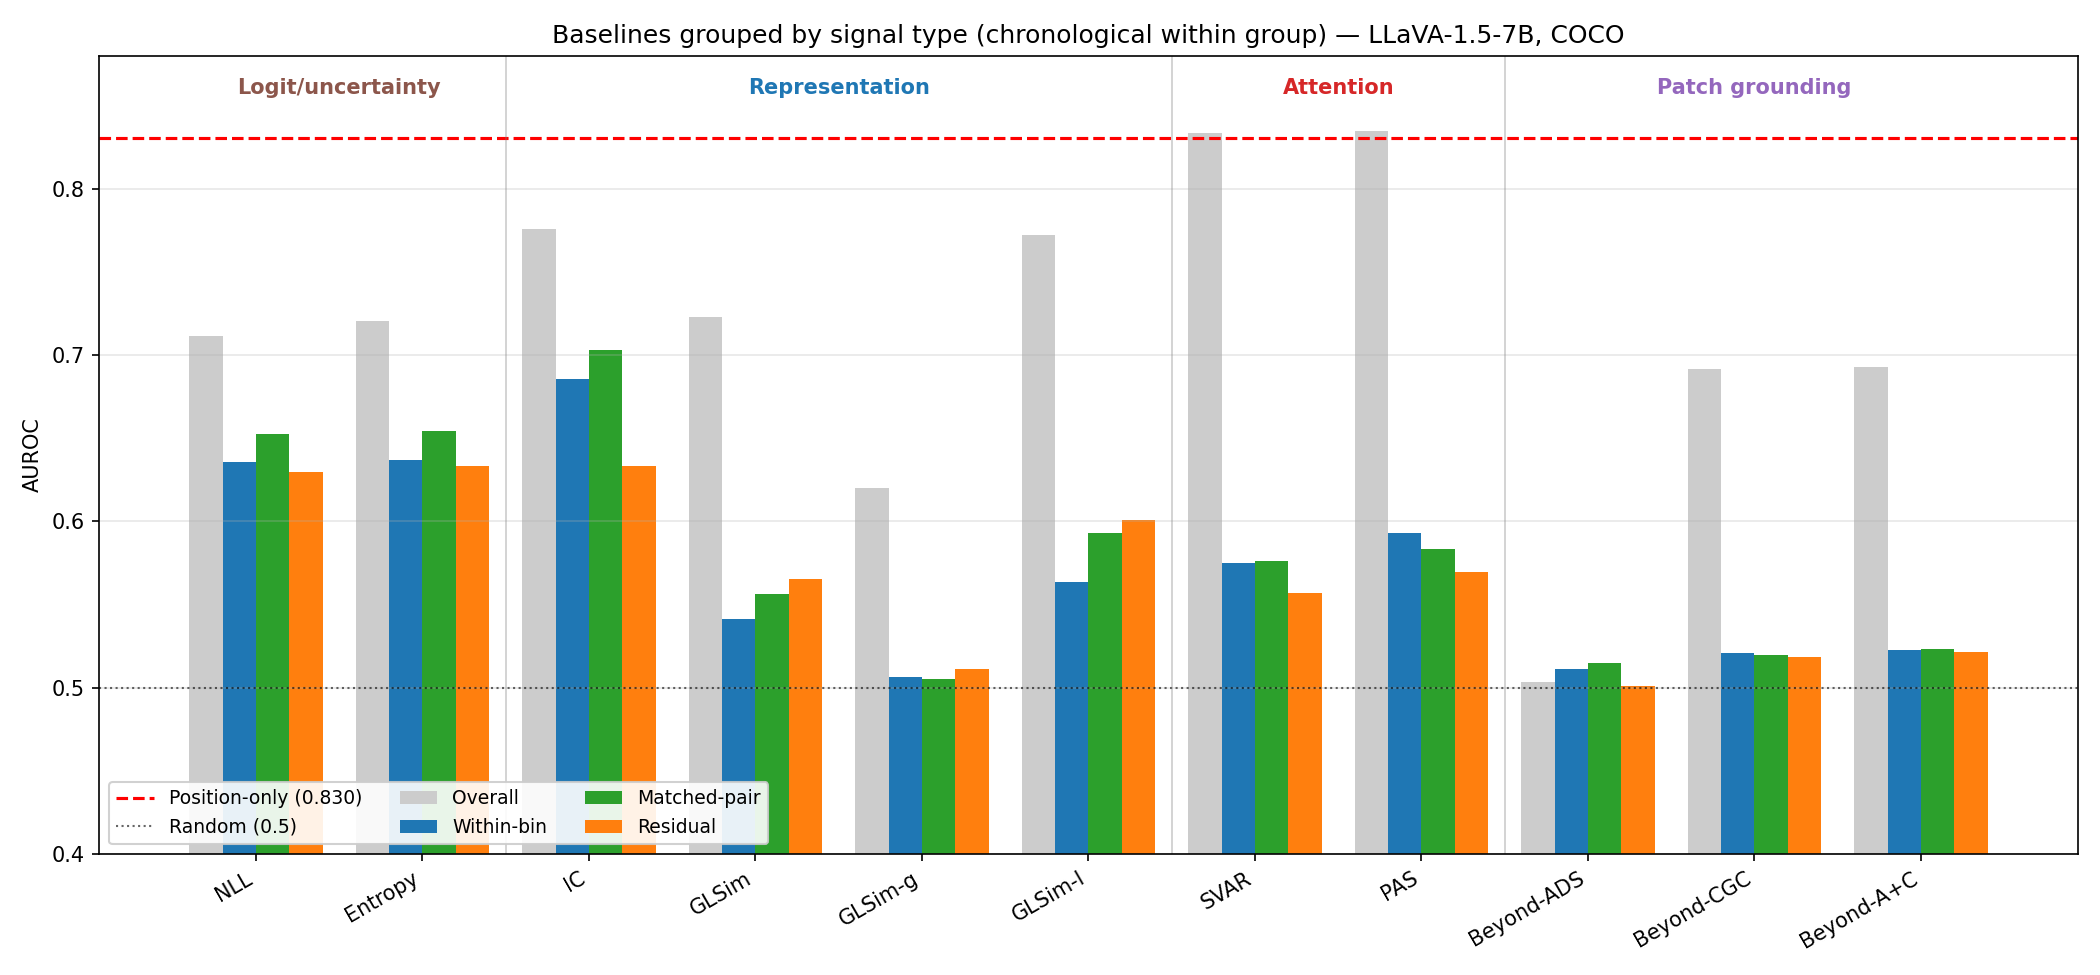
\includegraphics[width=0.95\textwidth]{assets/figures/fig_summary.png}
\caption{Overall vs.\ position-controlled AUROC by signal family. The dashed line marks position-only AUROC ($0.830$); the dotted line marks chance. PAS and SVAR look strongest in aggregate but collapse under position control.}
\label{fig:summary}
\end{figure*}

\begin{figure}[t]
\centering
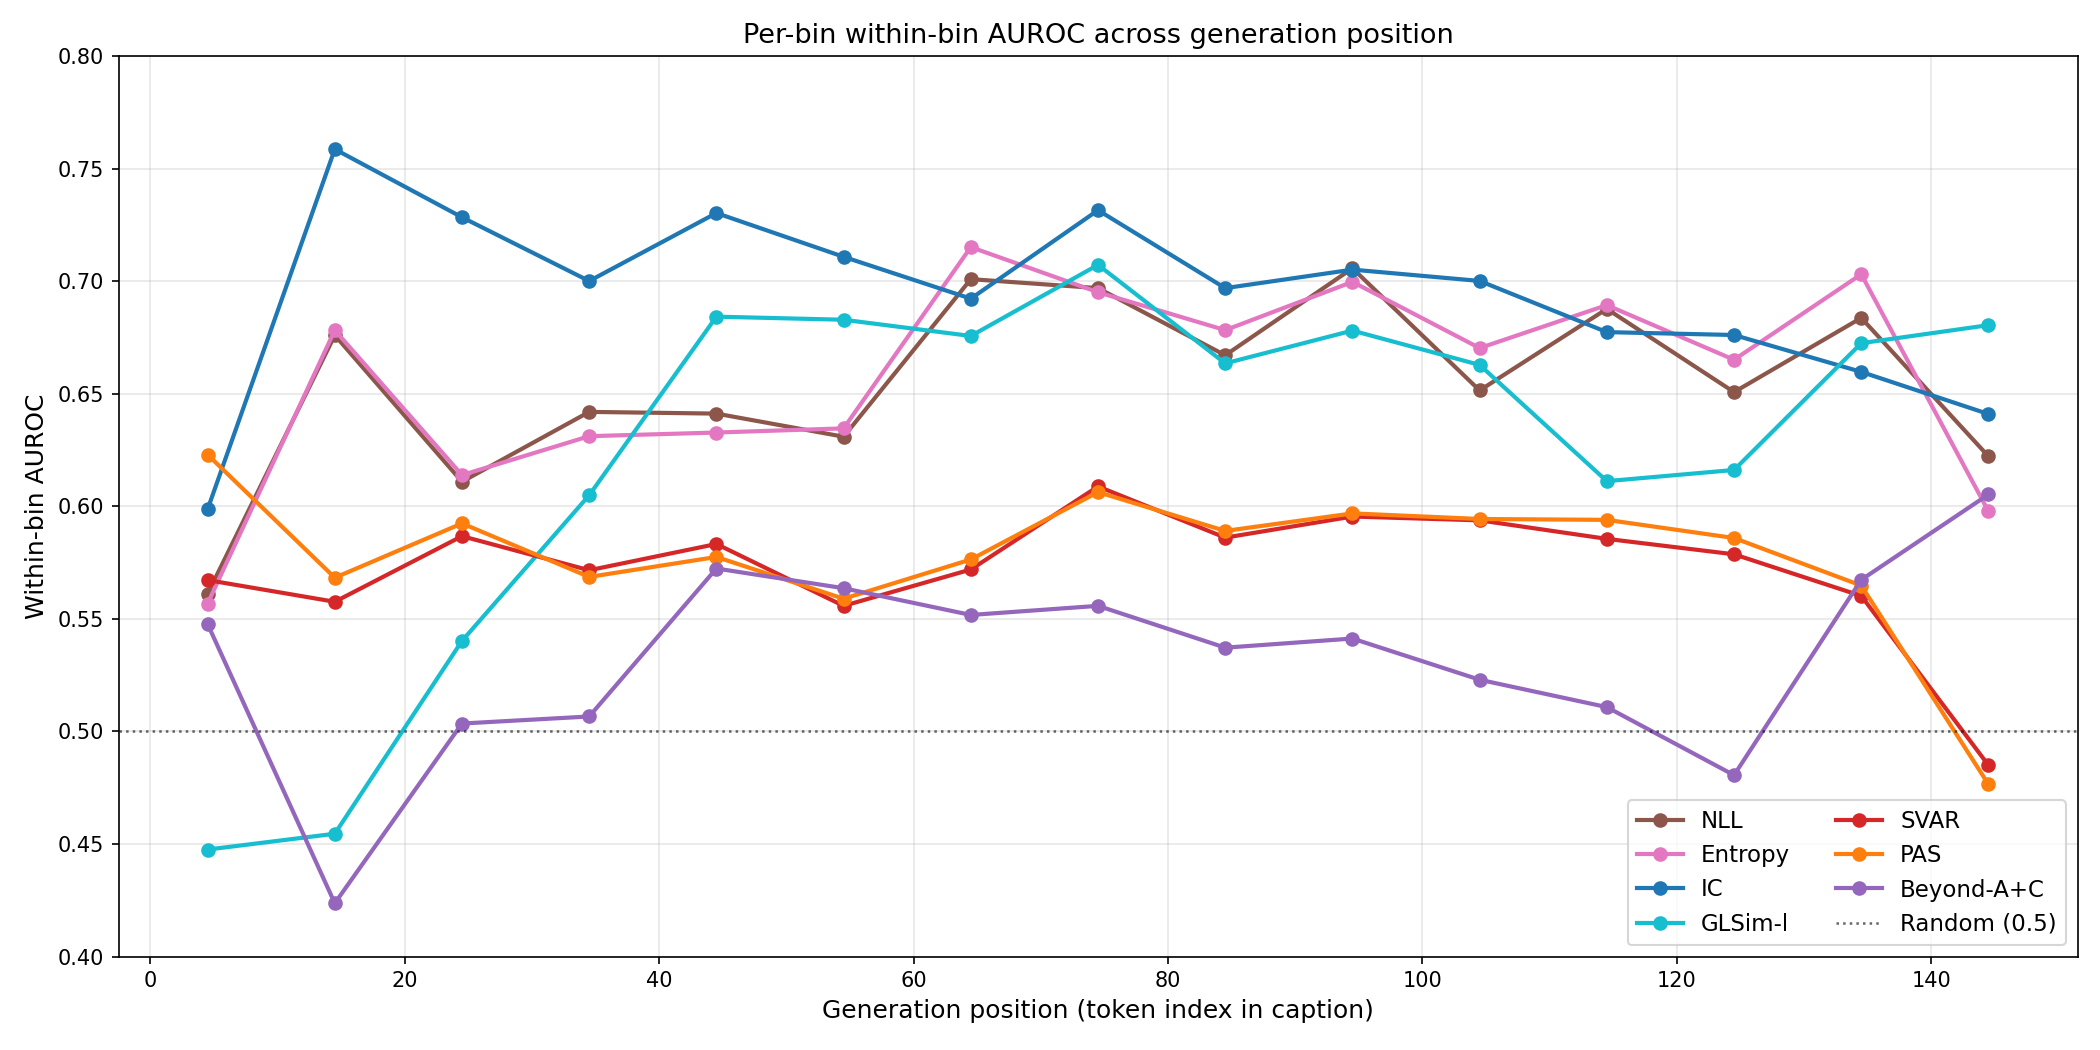
\includegraphics[width=\columnwidth]{assets/figures/fig_per_bin.png}
\caption{Within-bin AUROC across generation position. IC is consistently stronger than attention-mass scores; PAS/SVAR remain near $0.55$--$0.60$.}
\label{fig:perbin}
\end{figure}

\paragraph{A clean split between families.} Table~\ref{tab:main} and Figure~\ref{fig:summary} show that overall AUROC and position-controlled AUROC tell opposite stories for the attention family. PAS and SVAR have the two \emph{highest} overall AUROCs ($0.835$, $0.834$)---at or above the position-only floor---yet their within-bin AUROC is only $0.593$ and $0.575$. Expressed as retained above-chance signal, $(\text{within-bin}-0.5)/(\text{overall}-0.5)$, PAS keeps $28\%$ and SVAR $22\%$. By contrast, IC keeps $67\%$ ($0.686$ within-bin), entropy $62\%$, and NLL $64\%$. The fine-grained patch-grounding detectors (Beyond-*) are near chance on all position-controlled metrics. There is essentially no middle ground: methods retain either $\sim$$60$--$67\%$ or $\sim$$12$--$28\%$.

\paragraph{The split tracks signal source, not recency.} Ordering methods by proposal date (Figure~\ref{fig:summary}) shows the earliest representation method, IC, remains the strongest position-controlled detector, ahead of every later attention/grounding method. Improvements in overall AUROC over time largely reflect better fitting of the position prior, not new position-independent signal.

\paragraph{Per-position view.} Figure~\ref{fig:perbin} confirms the gap is consistent across positions: IC dominates in nearly every bin, whereas PAS/SVAR remain flat near $0.55$--$0.60$ throughout. The advantage of representation/uncertainty signals is not concentrated in a few easy bins.

\paragraph{What survives control is not simply ``more vision''.} The robust detectors are not the ones that most directly count image attention. Entropy and NLL read the output distribution, and IC reads whether internal visual representations support the object through a logit-lens style compatibility signal. These scores are imperfect, but they do not collapse as sharply when position is fixed. This suggests that the model contains object-relevant information, yet the information is not captured by coarse attention mass. In other words, the failure is not that LVLMs have no grounding signal; the failure is that attention mass is a poor stand-alone extractor of that signal.

\paragraph{The gap survives stronger matching.} Table~\ref{tab:strong-controls} reports the additional controls. The same-object-word matched AUROC is the most direct response to the possibility that detectors exploit object-frequency effects rather than grounding: IC, entropy, and NLL remain around $0.70$, while PAS and SVAR remain near $0.56$--$0.57$. Nonlinear residuals tell the same story. Cubic residual AUROC is $0.633$--$0.634$ for IC/entropy/NLL but only $0.558$ for PAS and $0.546$ for SVAR. Thus the detection split is not an artifact of the particular binning or residualization choice.

\begin{table}[t]
\centering
\scriptsize
\setlength{\tabcolsep}{3.0pt}
\begin{tabular}{lccc}
\toprule
Method & Same-word match & Cubic residual & Retained \\
\midrule
NLL & 0.698 & 0.630 & 0.93 \\
Entropy & 0.712 & 0.634 & 0.96 \\
IC & \textbf{0.716} & 0.633 & 0.78 \\
PAS & 0.569 & 0.558 & 0.21 \\
SVAR & 0.565 & 0.546 & 0.20 \\
GLSim-local & 0.615 & 0.600 & 0.42 \\
SinkDetect-global & 0.477 & 0.484 & -0.08 \\
SinkDetect-CLC & 0.592 & 0.550 & 0.64 \\
\bottomrule
\end{tabular}
\caption{Additional controls on saved per-object scores. Same-word match pairs hallucinated and grounded mentions of the same object word within $\pm5$ generated tokens. Retained is $(\mathrm{same\mbox{-}word}-0.5)/(\mathrm{overall}-0.5)$. Attention mass scores remain weak under object-category control.}
\label{tab:strong-controls}
\end{table}



\subsection{Stress Test: SinkDetect}
\label{sec:sinkdetect}

A natural objection is that attention \emph{shape}, as opposed to attention \emph{mass}, might carry position-independent grounding signal that prior attention detectors simply read too crudely. To test this directly we build SinkDetect, a detector designed to read shape.

\paragraph{Method.} Let $\tilde a_q$ be the object query's attention row restricted to the visual-token span, with detected sink columns removed and the remainder $L_1$-normalized to a distribution. SinkDetect scores $\tilde a_q$ along three axes. \emph{(i) Counterfactual visual grounding (CVG):} the negative divergence $-\mathrm{KL}(\tilde a_q \,\|\, \pi)$ and $-\mathrm{JSD}(\tilde a_q, \pi)$ from null distributions $\pi$ taken as the average instruction-token attention, a uniform distribution, and a local non-object null; closeness to a language-prior null is treated as evidence of hallucination. \emph{(ii) Concentration:} the entropy $H(\tilde a_q)$ and top-$k$ mass, testing whether attention is diffuse. \emph{(iii) Cross-layer consistency (CLC):} the generalized Jensen--Shannon divergence among the per-layer distributions, testing whether the attended region is stable across depth. Sinks are visual tokens with anomalously large pre-RoPE key norm that absorb attention mass without carrying semantics; removing them, together with an optional top-mass mask, forms a $2\times2$ purification ablation, each variant optionally recomputed on a no-RoPE branch. The full score set spans these axes $\times$ purification variants $\times$ per-layer/global aggregation. Crucially, because every distribution is $L_1$-normalized before scoring, total attention mass---the position-confounded quantity---is divided out by construction; SinkDetect therefore isolates \emph{shape}.

\paragraph{Result.} Despite this design, SinkDetect's best within-bin AUROC is $\approx$$0.50$, and its residual AUROC is $0.49$--$0.51$. Its highest \emph{overall} AUROC ($0.81$) again comes from a concentration score that correlates with position. Normalizing away mass does not help, because the confound also lives in the \emph{shape} of the normalized distribution: early tokens attend broadly (high entropy), late tokens attend narrowly, independent of grounding. We read this as evidence that the limitation is structural to attention-magnitude--derived signals on this model, not a failure of feature engineering: even purpose-built shape features, with sinks and dominant patches removed, recover no position-independent signal.

The SinkDetect result is useful precisely because it is a failed stress test. It removes the most obvious defects of attention-mass detectors: sink tokens, dominant visual patches, total mass, and RoPE-related ablations. Yet the best global score still comes from a feature whose distribution changes with decoding progress. This narrows the interpretation of the detection study. PAS and SVAR do not fail only because they use a crude scalar; a more careful hand-crafted attention shape also fails when forced to discriminate at comparable generation positions. A positive attention-based detector will likely need head-specific selection, learned verification, or external grounding constraints rather than another global average over visual rows.
